% CVPR 2022 Paper Template
% based on the CVPR template provided by Ming-Ming Cheng (https://github.com/MCG-NKU/CVPR_Template)
% modified and extended by Stefan Roth (stefan.roth@NOSPAMtu-darmstadt.de)

\documentclass[10pt,twocolumn,letterpaper]{article}

%%%%%%%%% PAPER TYPE  - PLEASE UPDATE FOR FINAL VERSION %%%%%%%%%
%\usepackage[review]{cvpr}      % To produce the REVIEW version
%\usepackage{cvpr}              % To produce the CAMERA-READY version
\usepackage[pagenumbers]{cvpr} % To force page numbers, e.g. for an arXiv version

% Include other packages here, before hyperref.
\usepackage{graphicx}
\usepackage{amsmath}
\usepackage{amssymb}
\usepackage{booktabs}
\usepackage{float}
\usepackage{arydshln}
\usepackage{enumitem}


% It is strongly recommended to use hyperref, especially for the review version.
% hyperref with option pagebackref eases the reviewers' job.
% Please disable hyperref *only* if you encounter grave issues, e.g. with the
% file validation for the camera-ready version.
%
% If you comment hyperref and then uncomment it, you should delete
% ReviewTempalte.aux before re-running LaTeX.
% (Or just hit 'q' on the first LaTeX run, let it finish, and you
%  should be clear).
\usepackage[pagebackref,breaklinks,colorlinks]{hyperref}


% Support for easy cross-referencing
\usepackage[capitalize]{cleveref}
\crefname{section}{Sec.}{Secs.}
\Crefname{section}{Section}{Sections}
\Crefname{table}{Table}{Tables}
\crefname{table}{Tab.}{Tabs.}

\raggedbottom
\begin{document}

%%%%%%%%% TITLE - PLEASE UPDATE %%%%%%%%%
\title{DLP Lab6: Conditional Generative Models}

\author{Yi-Hsiang Ho, 111550106
}
\maketitle

%%%%%%%%% BODY TEXT %%%%%%%%%

\section{Introduction}
\label{sec:intro}

In this lab, I implemented and evaluated a conditional generative model for
multi-label image synthesis using the \textbf{iclevr} dataset. The core
objective is to generate $64 \times 64$ images that accurately reflect
multiple object constraints (e.g., color and shape) through a denoising
process.

The implementation leverages several key technologies to achieve high-fidelity
conditional generation:
\begin{itemize}[itemsep=-3pt]
  \item \textbf{DDPM / DDIM}: Denoising Diffusion Probabilistic Models
    for the generative backbone, with Denoising Diffusion Implicit Models
    used for efficient sampling.
  \item \textbf{Cross-Attention Conditioning}: A mechanism to integrate
    multi-label embeddings into the U-Net architecture, allowing for precise
    spatial control.
  \item \textbf{Classifier-Free Guidance (CFG)}: A technique to enhance the
    alignment between the generated images and the input conditions.
\end{itemize}


\section{Implementation Details}
\label{sec:impl}

\subsection{Model Architecture}

The core of the generative model is a \textbf{Class-Conditioned U-Net}
implemented using the \verb|diffusers| library's
\verb|UNet2DConditionModel|. The architecture consists of several
downsampling and upsampling blocks with skip connections:
\begin{itemize}[itemsep=-3pt]
  \item \textbf{Downsampling}: Two \verb|DownBlock2D| followed by
  two \verb|CrossAttnDownBlock2D|.
  \item \textbf{Upsampling}: Two \verb|CrossAttnUpBlock2D| followed by
  two \verb|UpBlock2D|.
  \item \textbf{Channels}: The block output channels are (64, 128, 256, 512).
\end{itemize}

I utilized \textbf{Cross-Attention} conditioning for the final model. In this
setup, the class labels are passed as \verb|encoder_hidden_states|
to the U-Net. This allows the model to spatially attend to specific object
requirements during the denoising process. The code snippet is in
\cref{fig:model}.

\begin{figure}[H]
  \centering
  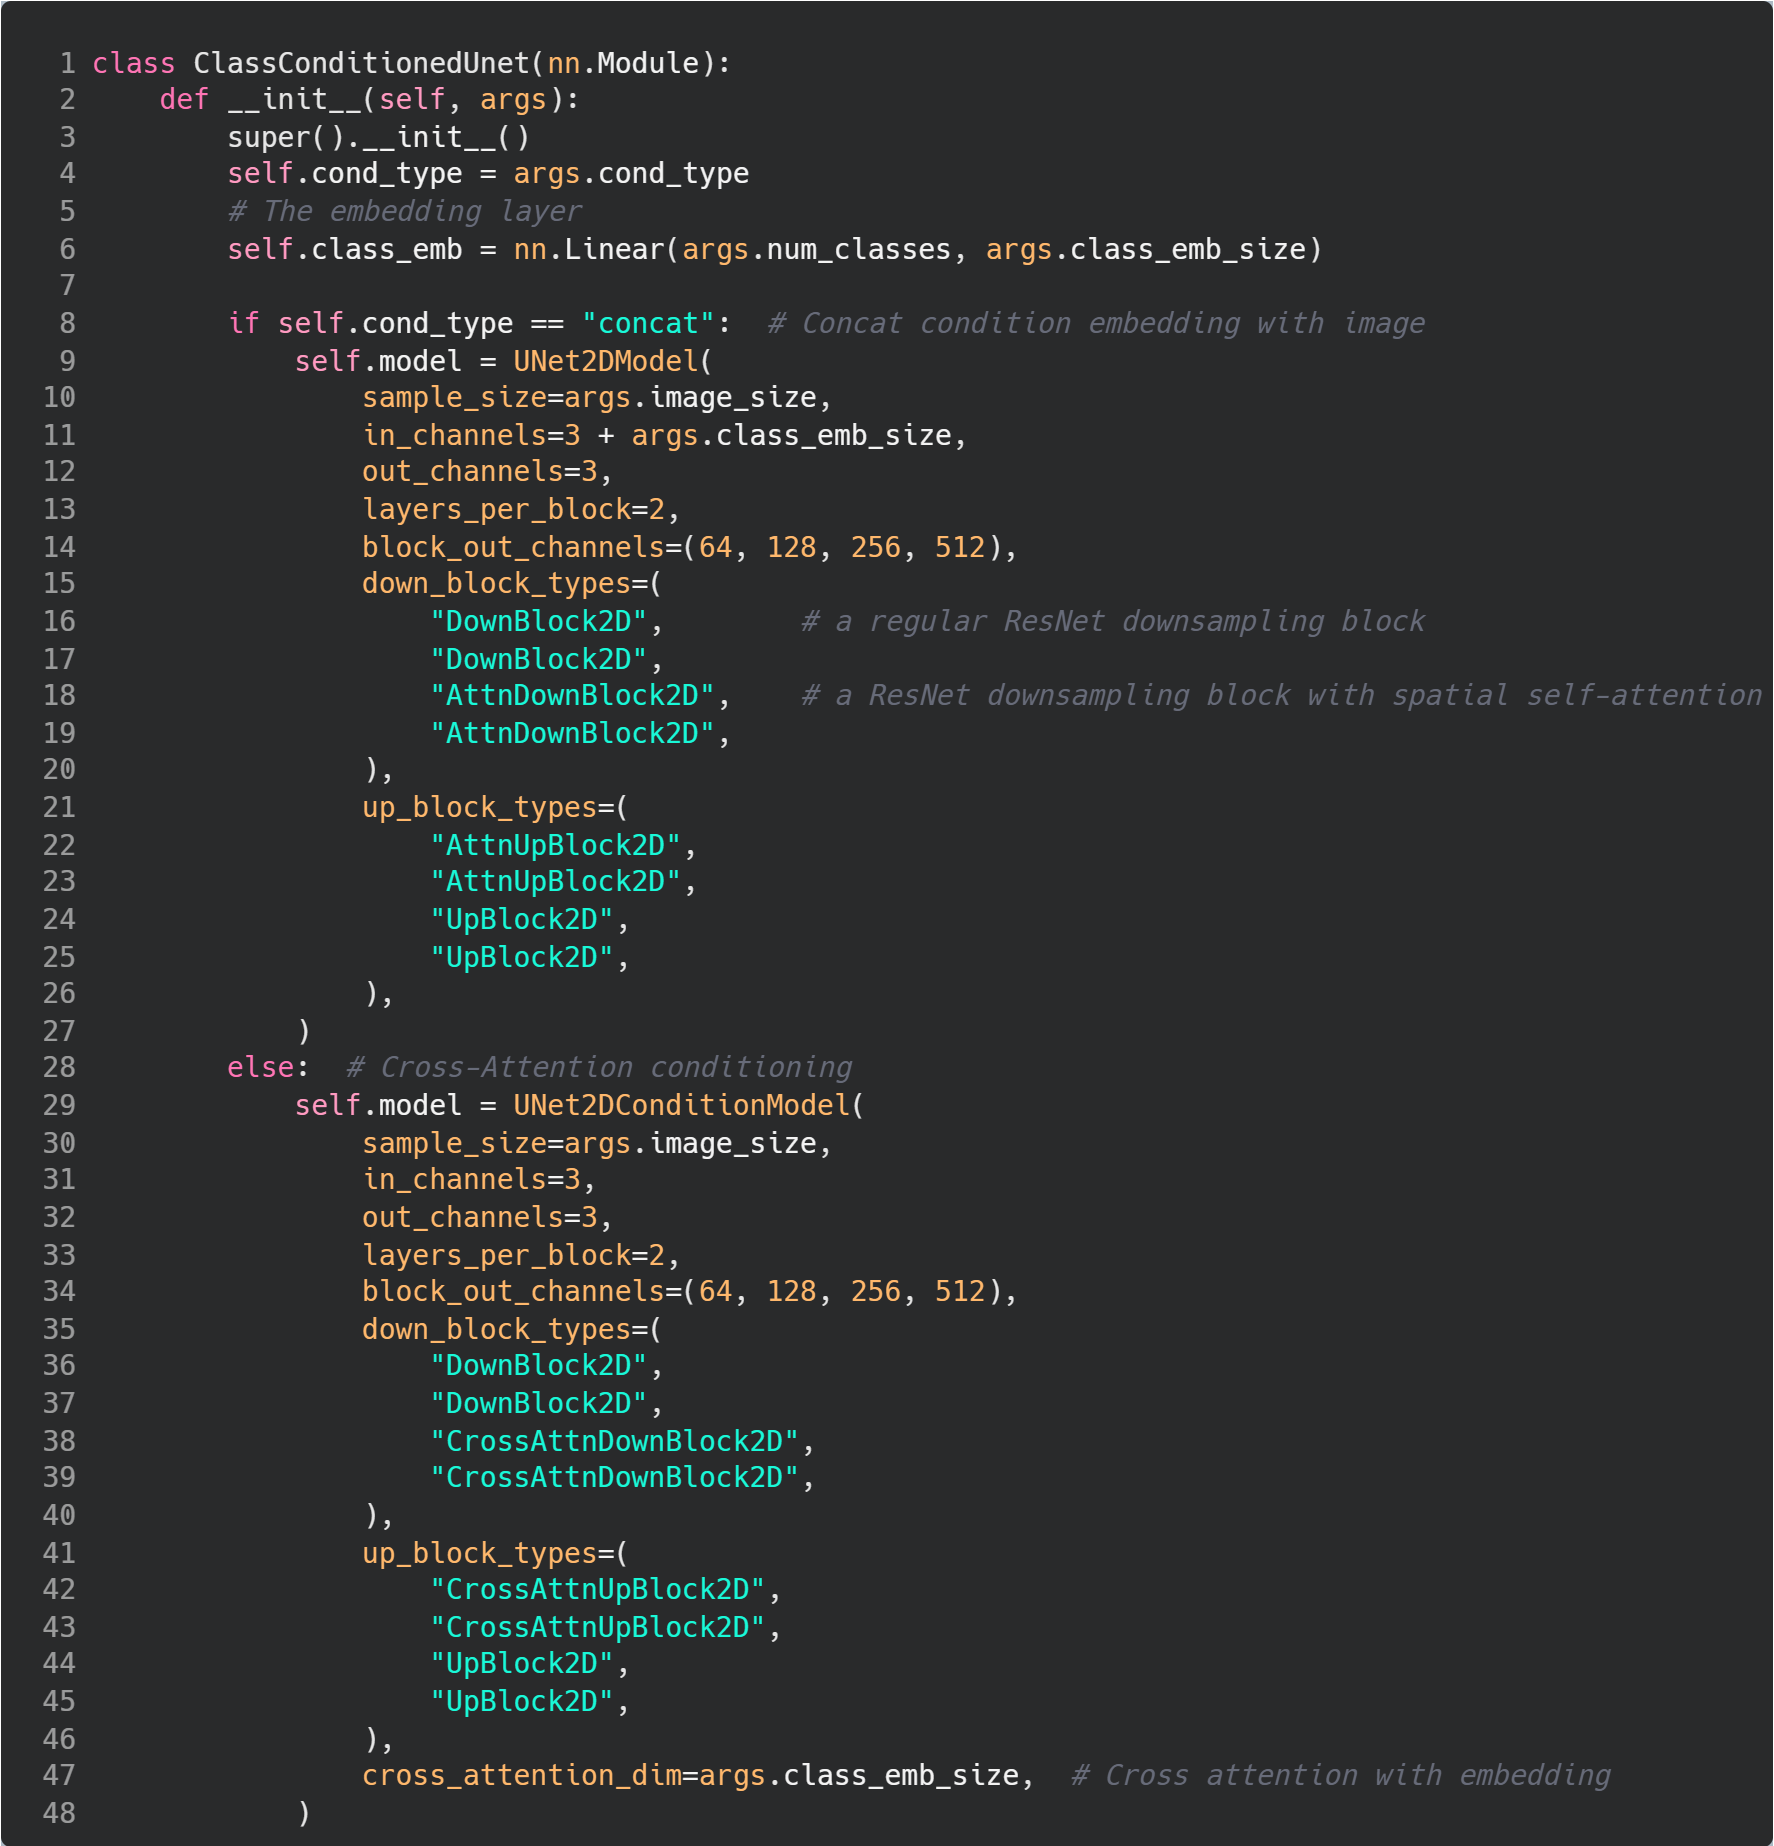
\includegraphics[width=1.0\linewidth]{assets/impl-model.png}
  \caption{\textbf{Model architecture}.}
  \label{fig:model}
\end{figure}

\subsection{Conditioning Mechanism}

The input labels are multi-hot vectors of size 24 (representing colors and
shapes). These labels are processed as follows and the implementation is in
\cref{fig:forward}:
\begin{enumerate}[itemsep=-3pt]
  \item The multi-hot label $L \in \{0, 1\}^{24}$ is projected through a
    \verb|nn.Linear| layer to a 256-dimensional embedding space.
  \item For Cross-Attention, this 256D vector is unsqueezed to
    form a sequence of length 1, acting as the context for the attention
    mechanism.
  \item For the Concatenation baseline, the vector is reshaped
    to $(256, 1, 1)$ and expanded to match the spatial resolution of the
    image $(256, 64, 64)$ before being concatenated with the noisy image input.
\end{enumerate}

\begin{figure}[H]
  \centering
  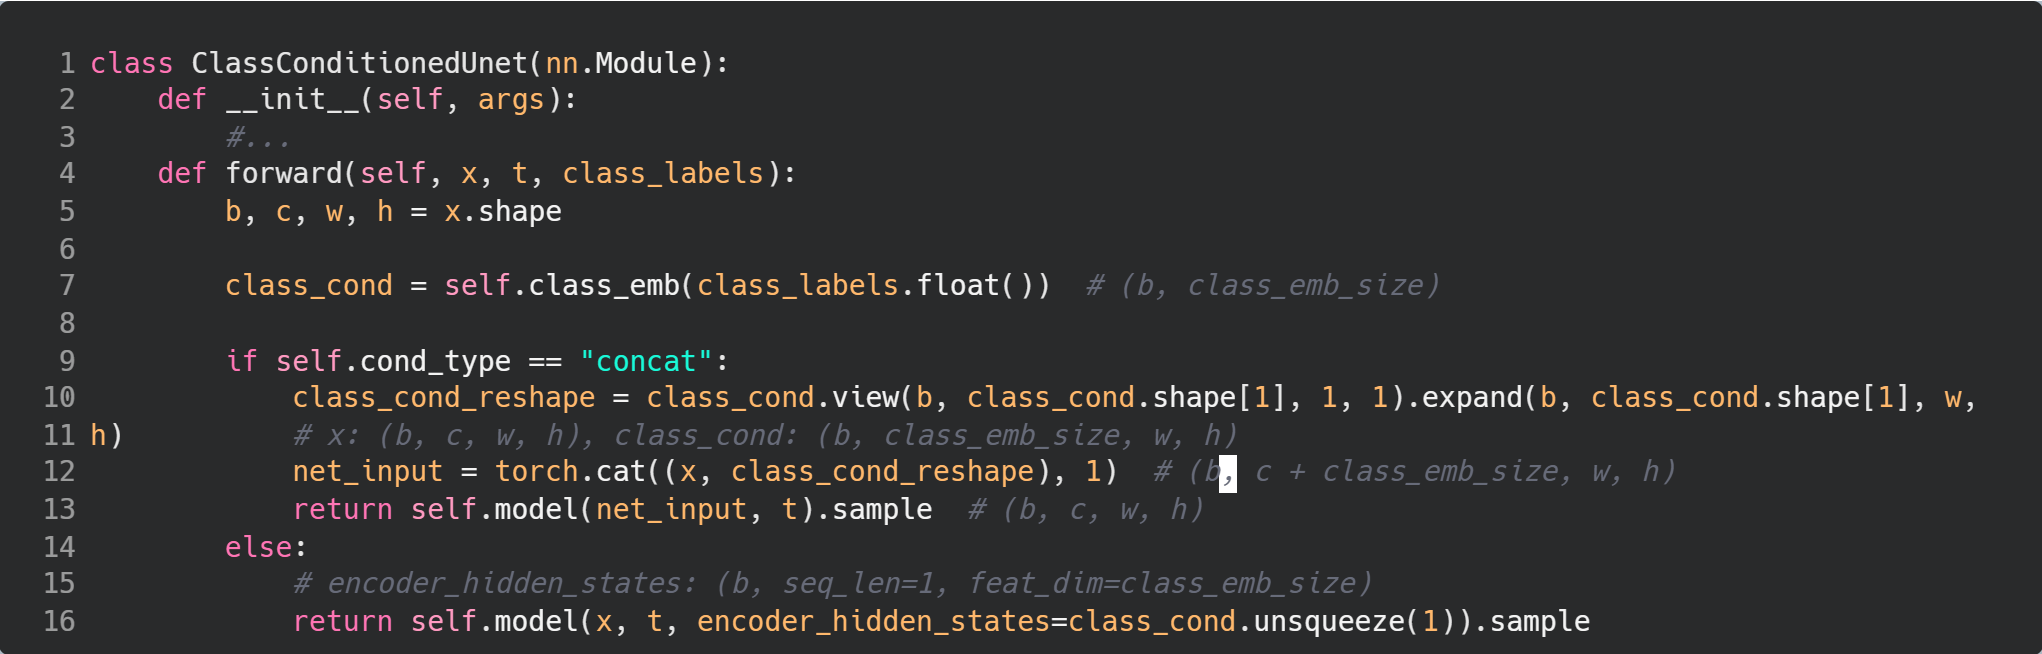
\includegraphics[width=1.0\linewidth]{assets/impl-forward.png}
  \caption{\textbf{Conditioning Mechanism}.}
  \label{fig:forward}
\end{figure}

\subsection{Training Procedure}

The model was trained for 200 epochs using the following hyperparameters:
\begin{itemize}[itemsep=-3pt]
  \item \textbf{Optimizer}: AdamW with a learning rate of $10^{-4}$ and
    weight decay of $0.01$.
  \item \textbf{Learning Rate Scheduler}: Cosine Annealing with
    $T_{max} = 200$.
  \item \textbf{Batch Size}: 64.
  \item \textbf{Loss Function}: Mean Squared Error (MSE) between the
    predicted noise $\hat{\epsilon}$ and the actual noise $\epsilon$.
  \item \textbf{Noise Schedule}: 1000 training timesteps with a
    \verb|scaled_linear| beta schedule.
\end{itemize}

To enable Classifier-Free Guidance (CFG), I implemented a joint training
strategy where the model learns both conditional and unconditional
distributions.

\subsection{Classifier-Free Guidance (CFG)}

To enhance the model's adherence to the multi-label conditions, I implemented
Classifier-Free Guidance (CFG). During training, I applied a 20\%
probability of setting the conditioning labels to a null vector (zero-hot). 

During inference, the final noise prediction $\hat{\epsilon}_\theta$ is
calculated by linearly extrapolating from the unconditional prediction
$\epsilon_\theta(x_t, \emptyset)$ towards the conditional prediction
$\epsilon_\theta(x_t, c)$ using a guidance scale $w$:
\begin{equation}
\hat{\epsilon}_\theta(x_t, c) = \epsilon_\theta(x_t, \emptyset) + w \cdot (\epsilon_\theta(x_t, c) - \epsilon_\theta(x_t, \emptyset))
\label{eq:cfg}
\end{equation}
The sampling implementation is illustrated in \cref{fig:impl-cfg}.

\begin{figure}[H]
  \centering
  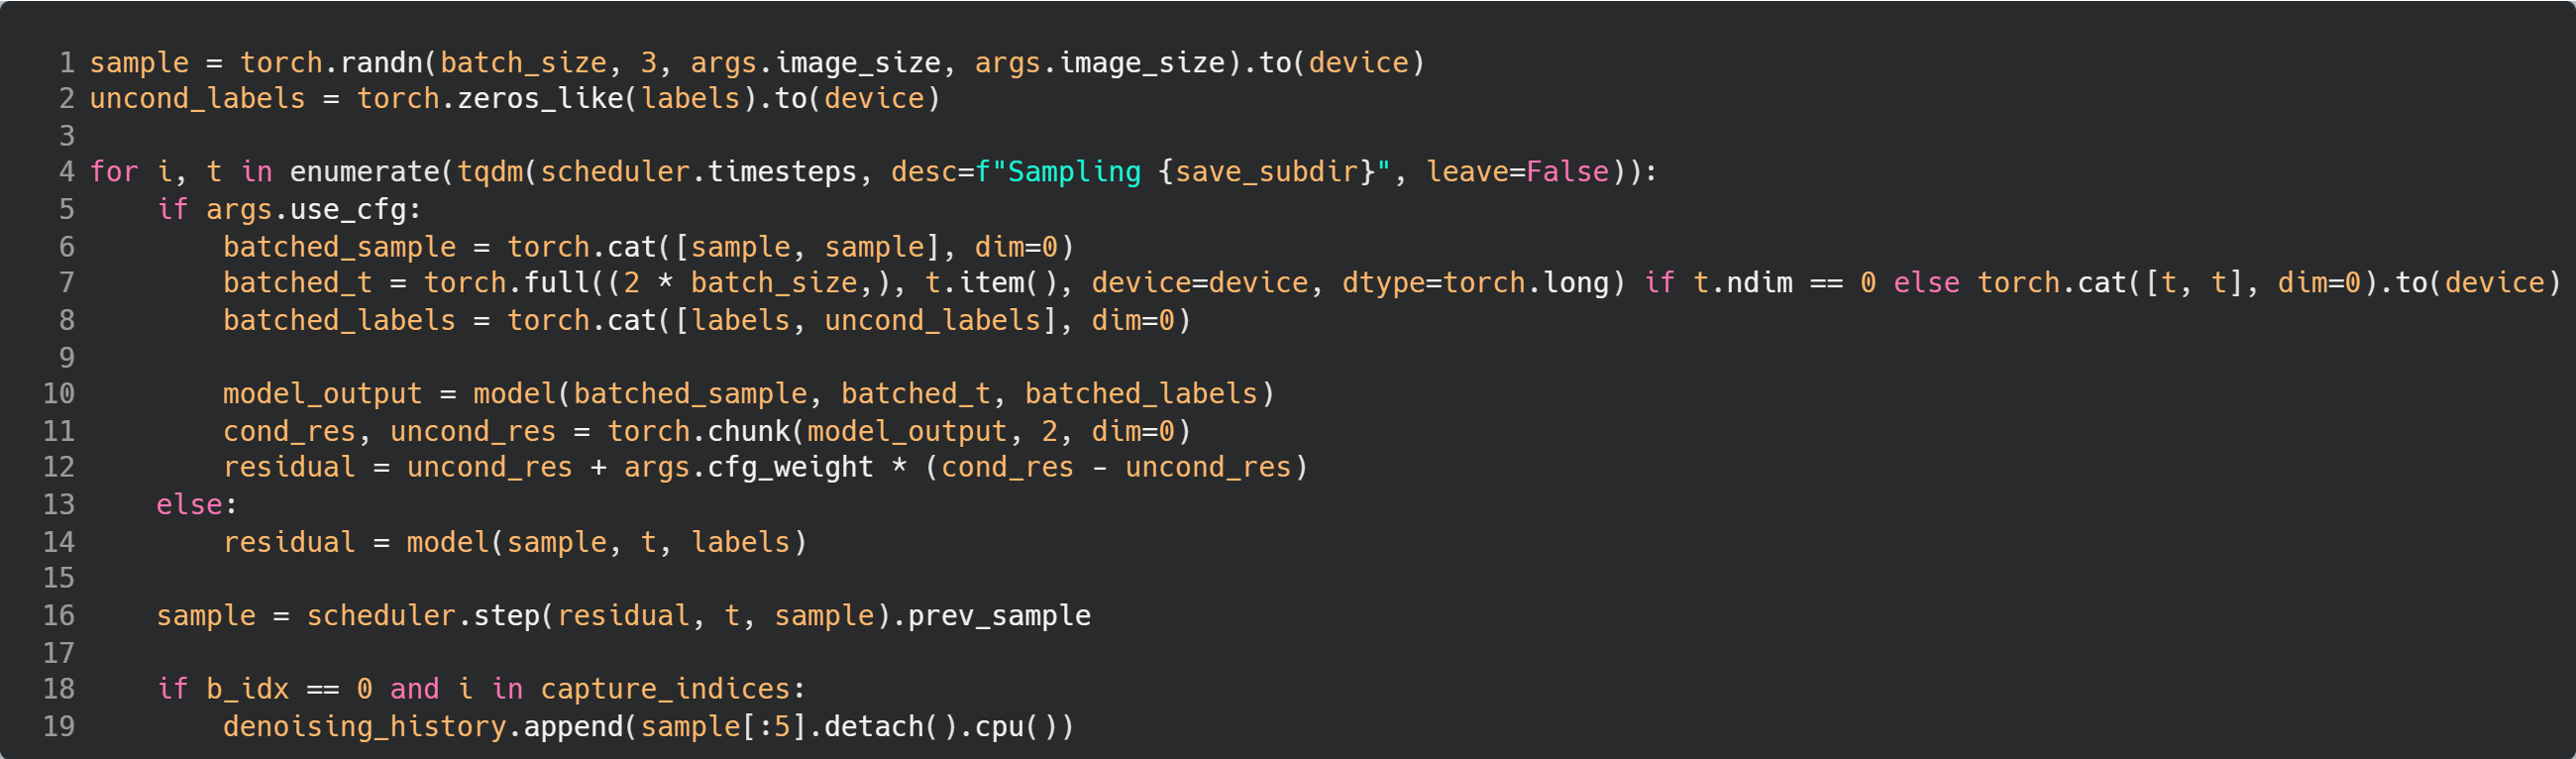
\includegraphics[width=1.0\linewidth]{assets/impl-cfg.png}
  \caption{\textbf{Classifier-Free Guidance}.}
  \label{fig:impl-cfg}
\end{figure}

\subsection{Denoising Diffusion Implicit Models (DDIM)}

For accelerated inference, I introduced Denoising Diffusion Implicit Models
(DDIM). Unlike the standard DDPM which requires 1000 sequential steps, DDIM
defines a non-Markovian forward process that allows for high-quality generation
in significantly fewer steps (e.g., 50--100 steps) by following a deterministic
sampling trajectory. The detailed implementation involves replacing the noise
scheduler from \verb|DDPMScheduler| to \verb|DDIMScheduler|, both of which are
provided by the \verb|diffusers| library.

While DDIM offers a nearly 50$\times$ speedup, I observed that it occasionally
resulted in slightly lower classification accuracy compared to the full DDPM
schedule for complex multi-label scenes. Consequently, while DDIM is supported for
fast prototyping, the results reported in \cref{sec:results} were obtained using
1000-step DDPM to ensure maximum fidelity.



\section{Results and Discussion}
\label{sec:results}

\subsection{Synthetic Image Grids}

The generated images for \verb|test.json| and \verb|new_test.json| are shown
in \cref{fig:grids}. The model successfully generates multiple objects with
correct colors and shapes.

\begin{figure}[H]
  \centering
  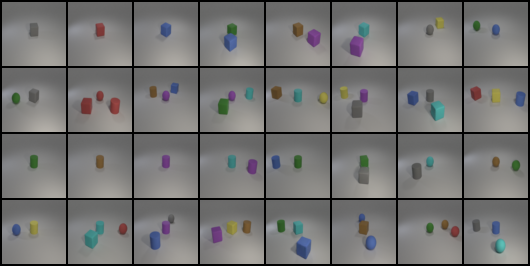
\includegraphics[width=1\linewidth]{assets/result-test_grid.png} \\[2mm]
  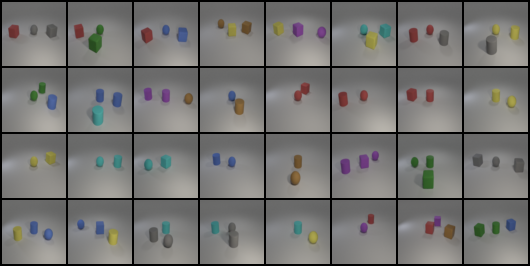
\includegraphics[width=1\linewidth]{assets/result-new_test_grid.png}
  \caption{\textbf{Synthetic Image Grids}. Up: \texttt{test.json}, Down: \texttt{new\_test.json}.  }
  \label{fig:grids}
\end{figure}

\subsection{Denoising Process}

The denoising process for the label set ["red sphere", "cyan cylinder",
"cyan cube"] is shown in \cref{fig:denoising}. The objects gradually emerge
from Gaussian noise as the timesteps decrease.

\begin{figure}[H]
  \centering
  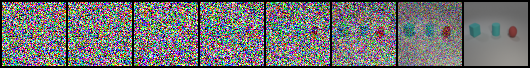
\includegraphics[width=\linewidth]{assets/result-denoising_process.png}
  \caption{\textbf{Denoising Process} for [red sphere, cyan cylinder, cyan cube].}
  \label{fig:denoising}
\end{figure}

\subsection{Classification Accuracy}

The classification accuracy was evaluated using a pre-trained evaluation
model. These results were achieved using DDPM with 1000 steps and a CFG
weight of 3.0.

\begin{table}[H]
  \centering
  \begin{tabular}{@{}lcc@{}}
    \toprule
    \textbf{Test Set} & \textbf{Accuracy} & \textbf{Inference Time} \\
    \midrule
    \verb|test.json|     & 0.8611 & 59.47s \\
    \verb|new_test.json| & 0.9048 & 59.68s \\
    \bottomrule
  \end{tabular}
  \caption{\textbf{Classification Accuracy} on test data.}
  \label{tab:acc}
\end{table}

The accuracy screenshots are provided in \cref{fig:acc}.

\begin{figure}[H]
  \centering
  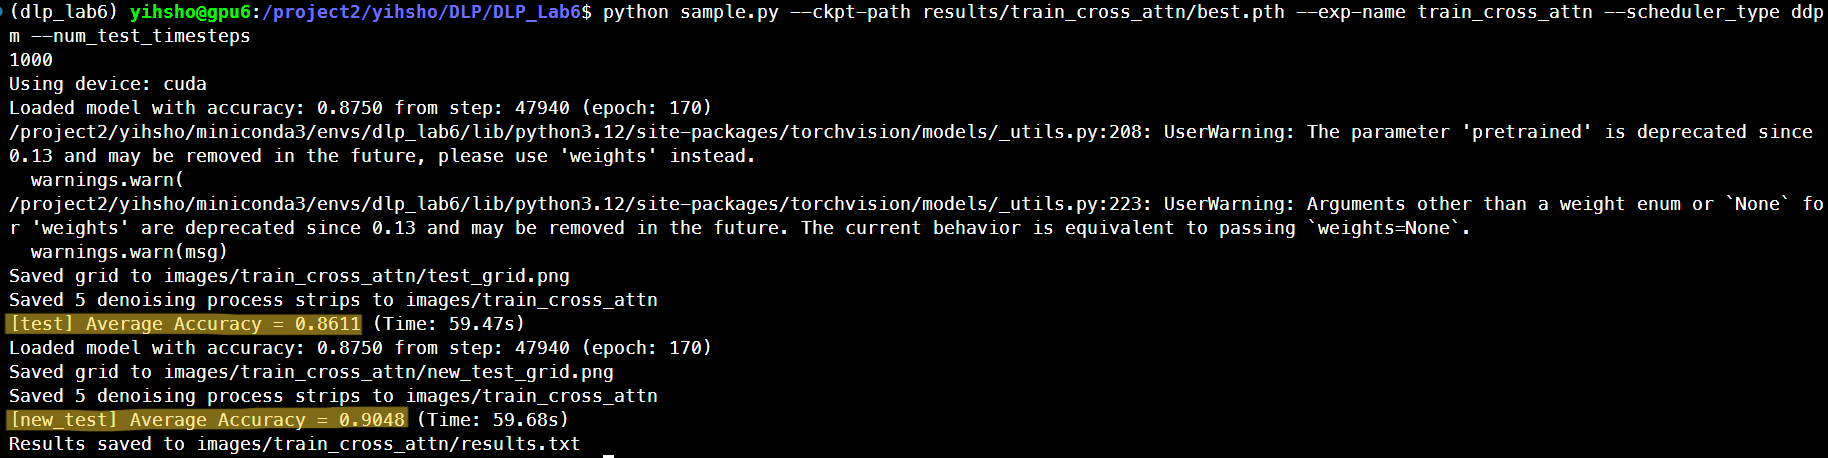
\includegraphics[width=\linewidth]{assets/result-acc.png}
  \caption{\textbf{Accuracy Screenshots}.}
  \label{fig:acc}
\end{figure}

\subsection{Discussion of Experiments}
\label{sec:discussion}

\subsection*{Conditioning Type}

I compared \textbf{Concatenation} and \textbf{Cross-Attention} for multi-label
conditioning. While Concatenation struggled to resolve spatial constraints
(approx. 0.43 accuracy), Cross-Attention allowed the U-Net to attend to
labels at multiple scales, achieving significantly higher accuracy (over 0.86).
Results are summarized in \cref{tab:conditioning}.

\begin{table}[H]
  \centering
  \small
  \begin{tabular}{@{}lcc@{}}
    \toprule
    \textbf{Conditioning Type} & \textbf{Test Acc} & \textbf{New Test Acc} \\
    \midrule
    Concatenation   & 0.4306 & 0.5595 \\
    Cross-Attention & \textbf{0.8611} & \textbf{0.9048} \\
    \bottomrule
  \end{tabular}
  \caption{\textbf{Ablation Study: Conditioning Mechanism} (DDPM, 1000 steps,
    CFG: 3.0, Beta: scaled linear). The highest accuracy is marked in bold.}
  \label{tab:conditioning}
\end{table}

\subsection*{Classifier-Free Guidance (CFG) Weight}

The guidance scale $w$ balances fidelity and diversity. These experiments
used DDIM with 50 steps to analyze the trend (\cref{tab:cfg-ablation}).
\begin{itemize}[itemsep=-3pt]
  \item $w=1.0$: Results in lower clarity and weaker alignment with input
    labels.
  \item $w=2.0$: Optimal balance for conditional fidelity and image quality.
  \item $w \ge 5.0$: Causes "guidance collapse," where over-saturation and
    shape distortion significantly degrade scores. Notably, when $w > 8$,
    the model begins to ignore the input conditions entirely as the guidance
    signal overpowers the generative process.
\end{itemize}
Visual comparisons are in \cref{fig:cfg}.

\begin{table}[H]
  \centering
  \small
  \begin{tabular}{@{}ccc@{}}
    \toprule
    \textbf{CFG Weight ($w$)} & \textbf{Test Acc} & \textbf{New Test Acc} \\
    \midrule
    w/o CFG & 0.7639 & 0.8571 \\
    1.0 & 0.6806 & 0.8333 \\
    2.0 & \textbf{0.7778} & \textbf{0.8929} \\
    3.0 & \textbf{0.7778} & 0.8452 \\
    5.0 & 0.6944 & 0.5952 \\
    8.0 & 0.2917 & 0.4167 \\
    \bottomrule
  \end{tabular}
  \caption{\textbf{Ablation Study: Classifier-Free Guidance Weight} (DDIM,
    50 steps, Beta: scaled linear). The highest accuracy is marked in bold.}
  \label{tab:cfg-ablation}
\end{table}

\begin{figure}[H]
  \centering
  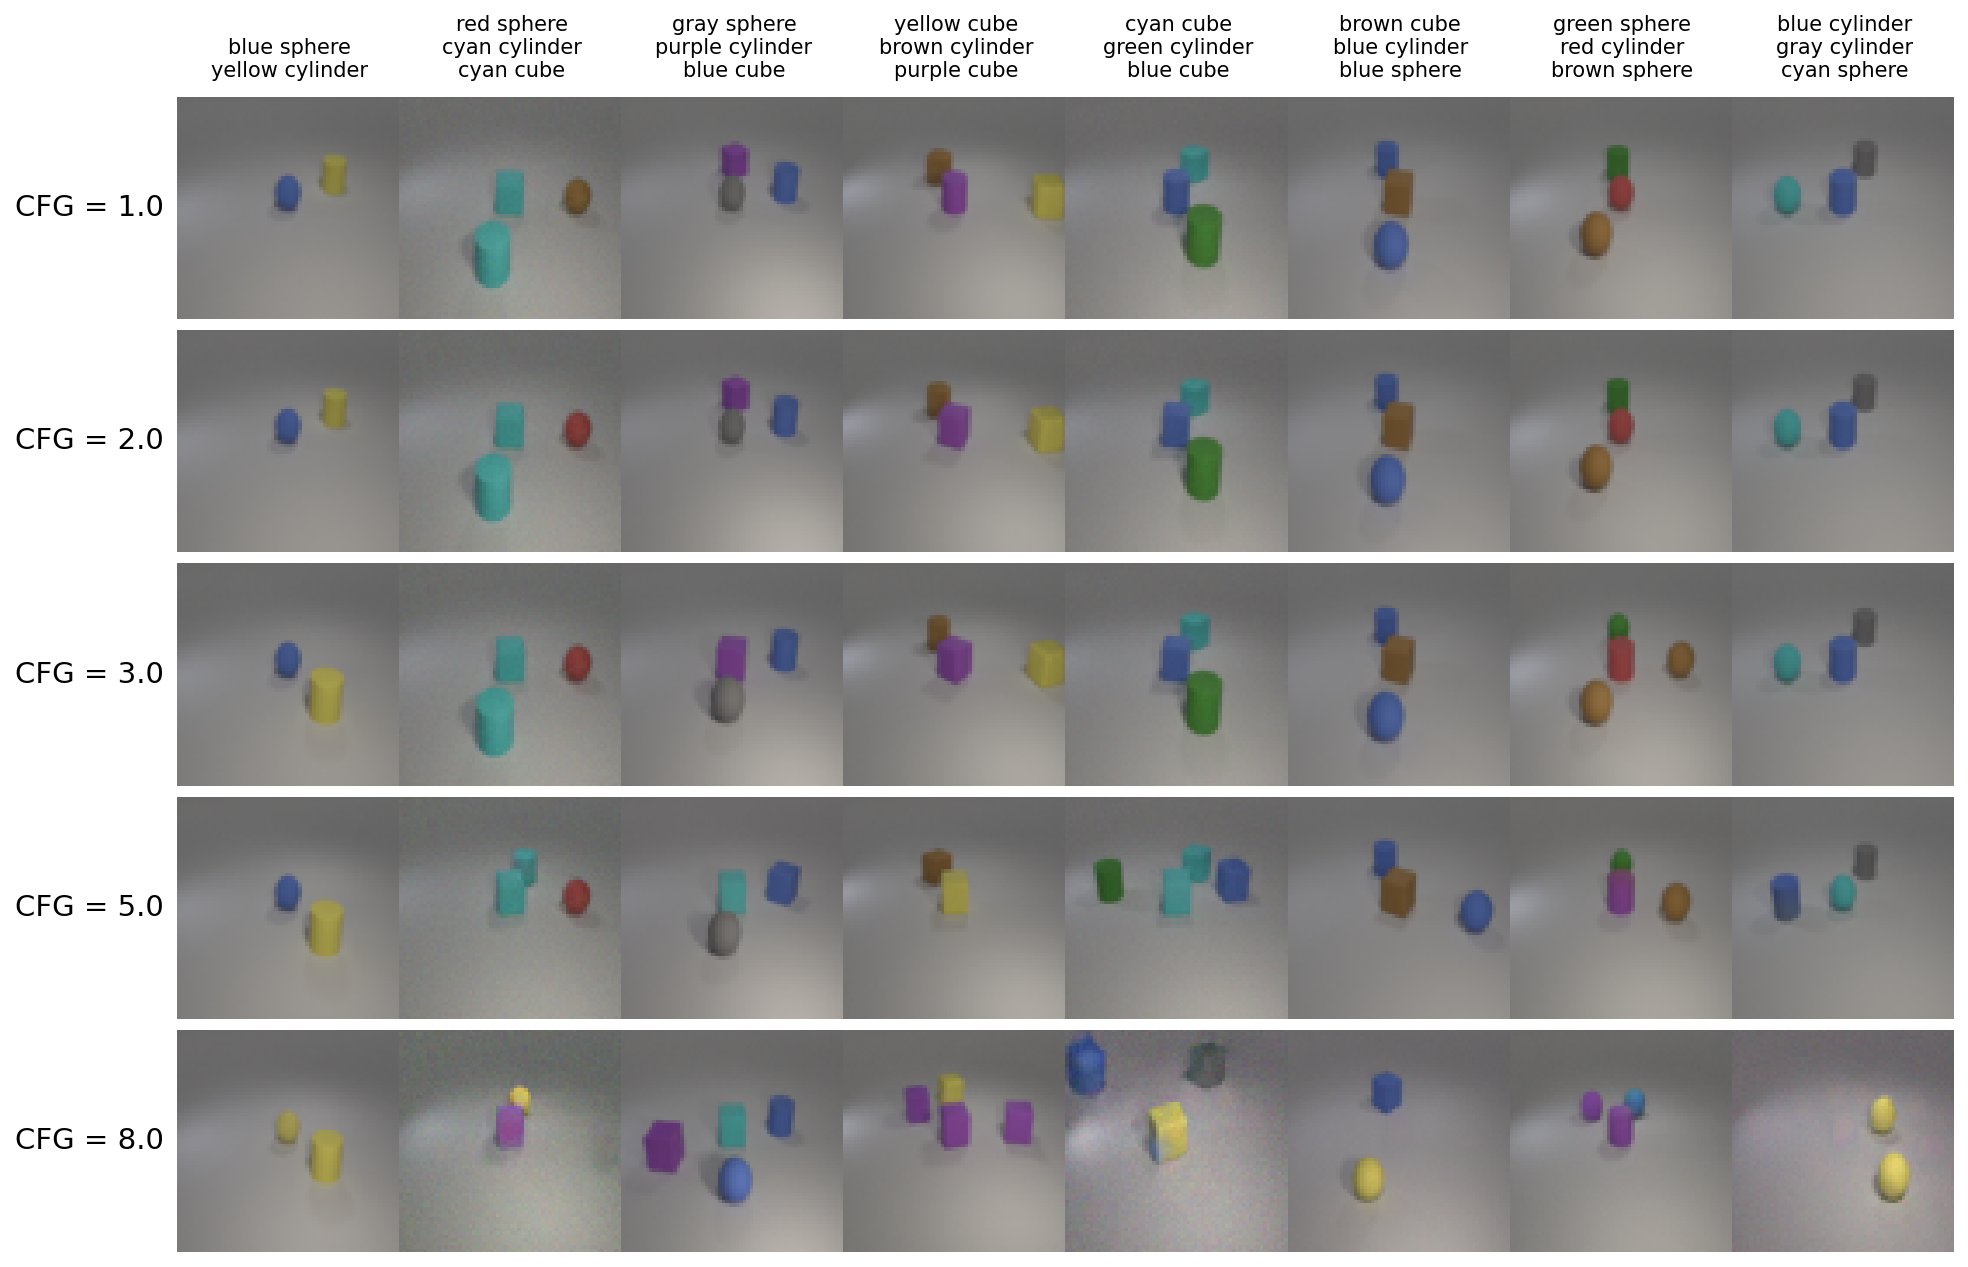
\includegraphics[width=\linewidth]{assets/abl-cfg_compare.png}
  \caption{\textbf{Classifier-Free Guidance Weight}.}
  \label{fig:cfg}
\end{figure}

\subsection*{Beta Schedule Analysis}

The noise schedule dictates the pace of information retrieval
(\cref{tab:beta-ablation}). While \textbf{Linear} destroys
structure too rapidly, \textbf{Scaled Linear} and \textbf{Squared Cosine}
provide a more gradual transition. Squared Cosine achieved the highest
accuracy as it preserves structural information more effectively during
the early stages of denoising.

\begin{table}[H]
  \centering
  \small
  \begin{tabular}{@{}lcc@{}}
    \toprule
    \textbf{Beta Schedule} & \textbf{Test Acc} & \textbf{New Test Acc} \\
    \midrule
    Linear          & 0.6944 & 0.8095 \\
    Scaled Linear   & 0.7639 & 0.8095 \\
    Squared Cosine  & \textbf{0.7917} & \textbf{0.8333} \\
    \bottomrule
  \end{tabular}
  \caption{\textbf{Ablation Study: Beta Schedule} (DDIM, 50 steps, CFG=3.0).
    The highest accuracy is marked in bold.}
  \label{tab:beta-ablation}
\end{table}

\subsection*{DDPM vs. DDIM Sampling}

We evaluated the speed-accuracy trade-off between DDPM and DDIM
(\cref{tab:steps-ablation}).
\begin{itemize}[itemsep=-3pt]
  \item \textbf{DDPM (1000 steps)}: Achieved the peak performance with
    \textbf{0.8611} and \textbf{0.9048} accuracy. The 1000-step trajectory
    provides superior stability for resolving multi-label spatial constraints,
    though it requires significantly more time ($\sim$119s).
  \item \textbf{DDIM (10--100 steps)}: Offers a substantial speedup, with
    10 steps taking only 2.48s. While efficient, it results in lower accuracy.
    Notably, increasing DDIM steps beyond 50 did not improve results, suggesting
    that the model benefits from the stochastic nature of DDPM for fine error
    correction.
\end{itemize}

\begin{table}[H]
  \centering
  \small
  \begin{tabular}{@{}lcccc@{}}
    \toprule
    \textbf{Scheduler} & \textbf{Steps} & \textbf{Test Acc} & \textbf{New Test Acc} & \textbf{Total Time} \\
    \midrule
    DDIM & 10    & 0.7778 & 0.8452 & 2.48s \\
    DDIM & 25    & 0.7778 & 0.8571 & 4.41s \\
    DDIM & 50    & 0.7778 & 0.8452 & 7.14s \\
    DDIM & 100   & 0.7222 & 0.8452 & 12.99s \\
    DDPM & 1000  & \textbf{0.8611} & \textbf{0.9048} & 119.20s \\
    \bottomrule
  \end{tabular}
  \caption{\textbf{Ablation Study: Sampling Steps and Scheduler} (CFG: 3.0,
    Beta: scaled linear). The highest accuracy is marked in bold.}
  \label{tab:steps-ablation}
\end{table}

\section{Conclusion}

In this lab, I successfully implemented a conditional DDPM/DDIM model for
multi-label image generation. By utilizing Cross-Attention and Classifier-Free
Guidance, the model achieved high classification accuracy and produced visually
plausible images on the iclevr dataset. The experiments highlighted the importance
of conditioning mechanisms and guidance weights in controlling the generative
process.

\end{document}